\newpage
 \begin{center}
 \begin{Large}
 \textbf{
% Gaussian Process Dynamical Systems\\
 Appendix
 } \\
 \end{Large}
% \noindent \newline
% \textbf{Andreas Damianou, Michalis Titsias, Neil Lawrence}
 \end{center}
\appendix







\section{Calculating $\hat{\mathcal{F}_d}(q, \boldsymbol \theta)$}

We have:
\begin{equation}
\hat{\mathcal{F}_d} \geq
	\log \int e^{\la \log N \left( \bfy_d | \bfa_d, \beta^{-1} I_d \right) \ra_{q(X)}}
		p(\bfu_d) \intd \bfu_d -\mathcal{A} .
\end{equation}

with:

\begin{equation}
\label{boundFIntegral}
\int e^{\la \log N \left( \bfy_d | \bfa_d, \beta^{-1} I_d \right) \ra_{q(X)}}
		p(\bfu_d) d\bfu_d = 
\int e^{\la \log N \left( \bfy_d | \bfa_d, \beta^{-1} I_d \right) \ra_{q(X)} + \log p(\bfu_d)}
		d\bfu_d
\end{equation}

The expectation involved in the quantity above is calculated as:
\begin{align}
\la \log N \left( \bfy_d | \bfa_d, \beta^{-1} I_d \right) \ra_{q(X)} = {}& 
- \frac{N}{2} \log (2 \pi) - \frac{1}{2} \log \vert \beta^{-1} I_d \vert 
- \frac{1}{2} Tr \la \beta I_d \left( \bfy_d - \bfa_d) (\bfy_d - \bfa_d \right)^\T \ra \nonumber \\
={}&
- \frac{N}{2} \log ( 2 \pi ) - \frac{1}{2} \log \vert \beta^{-1} I_d \vert 
- \frac{1}{2} Tr \left[ \beta I_d \left( \bfy_d \bfy_d^\T - 
2 \bfy_d \la \bfa_d^\T \ra + \la \bfa_d \bfa_d^\T \ra \right) \right] \label{boundFExpectation1}
\end{align}

but $\la \bfa_d \ra = \la K_{NM} \ra K_{MM}^{-1} \bfu_d$ and 
$\la \bfa_d \bfa_d^\T \ra = \la K_{NM} \ra K_{MM}^{-1} \bfu_d \bfu_d^\T K_{MM}^{-1} \la K_{NM}^\T \ra$ ($K_{MM}$ is symmetric so it's equal to its transpose), so \eqref{boundFExpectation1} now becomes:
\begin{align}
\la \log N \left( \bfy_d | \bfa_d, \beta^{-1} I_d \right) \ra_{q(X)} = {}&
- \frac{N}{2} \log (2 \pi) - \frac{1}{2} \log \vert \beta^{-1} I_d \vert \nonumber \\
{}& - \frac{1}{2} Tr \left[
	\beta I_d \left( \bfy_d \bfy_d^\T - 2 \bfy_d \bfu_d^\T K_{MM}^{-1} \la K_{NM}^\T \ra + 
	\bfu_d^\T K_{MM}^{-1} \la K_{NM}^\T K_{NM} \ra K_{MM}^{-1} \bfu_d \right) \right]
\end{align}

We now set:
\begin{equation*}
\Psi_0 = Tr(\langle \mathit{K_{NN}} \rangle_{q(\mathit{X})}) \;, \;\;
\Psi_1 = \langle \mathit{K_{NM}} \rangle_{q(\mathit{X})} \;, \;\;
\Psi_2 = \langle \mathit{K_{MN}} \mathit{K_{NM}} \rangle_{q(\mathit{X})}
\end{equation*}

and we get:

\begin{align}
{}& \la \log N \left( \bfy_d | \bfa_d, \beta^{-1} I_d \right) \ra_{q(X)} = \nonumber \\
{}& \;\;\;\;\;\;
	 - \frac{N}{2} \log (2 \pi) - \frac{1}{2} \log \vert \beta^{-1} I_d \vert \nonumber \\
{}& \;\;\;\;\;\; 
	- \frac{1}{2} Tr \left[
	\beta I_d \left( \bfy_d \bfy_d^\T - 2 \bfy_d \bfu_d^\T K_{MM}^{-1} \Psi_1^\T + 
	\bfu_d^\T K_{MM}^{-1} \Psi_2 K_{MM}^{-1} \bfu_d \right) \right]
\end{align}

We now add $\log p(\bfu_d)$ so as to get the full quantity which is integrated in \eqref{boundFIntegral}. Thus, we use \eqref{priorF2} and we get:

\begin{align}
{}& \la \log N \left( \bfy_d | \bfa_d, \beta^{-1} I_d \right) \ra_{q(X)} + \log p(\bfu_d) = \nonumber \\
{}& \;\;\;\;\;\;
	 - \frac{N}{2} \log (2 \pi) - \frac{1}{2} \log \vert \beta^{-1} I_d \vert \nonumber \\
{}& \;\;\;\;\;\; 
	- \frac{1}{2} Tr \left[
	\beta I_d \left( \bfy_d \bfy_d^\T - 2 \bfy_d \bfu_d^\T K_{MM}^{-1} \Psi_1^\T + 
	\bfu_d^\T K_{MM}^{-1} \Psi_2 K_{MM}^{-1} \bfu_d \right) \right] \nonumber \\
{}& \;\;\;\;\;\;
	- \frac{M}{2} \log (2 \pi ) - \frac{1}{2} \log \vert K_{MM} \vert - 
	\frac{1}{2} Tr \left( K_{MM}^{-1} \bfu_d \bfu_d^\T \right)  \label{boundFIntegral2}
\end{align}

By completing the square, \eqref{boundFIntegral2} can be rewritten as:
\begin{align}
{}& \la \log N \left( \bfy_d | \bfa_d, \beta^{-1} I_d \right) \ra_{q(X)} + \log p(\bfu_d) = \nonumber \\
{}& \;\;\;\;\;\;
  - \frac{N}{2} \log (2 \pi) - \frac{1}{2} \log \vert \beta^{-1} I_d \vert
  - \frac{1}{2} \log \vert K_{MM} \vert \nonumber \\
 {}& \;\;\;\;\;\;
  - \frac{\beta}{2} \bfy_d^\T \bfy_d + \frac{1}{2} m^\T S^{-1} m + \frac{1}{2} \log \vert S \vert
  + \log N(\bfu_d | m, S) \label{boundFIntegral3}
\end{align}
where
\begin{align}
S = {}& \left( \beta K_{MM}^{-1} \Psi_2 K_{MM}^{-1} + K_{MM}^{-1} \right)^{-1} \label{boundFVarS} \mbox{\;\;\;\; and} \\
m = {}& \beta S K_{MM}^{-1} \Psi_1^\T \bfy_d \label{boundFVarm}
\end{align}

We can now obtain the final expression for \eqref{boundFIntegral} by simply putting the quantity of \eqref{boundFIntegral3} on the exponent and integrating. By doing so, we get:

\begin{align}
{}& \int e^{\la \log N \left( \bfy_d | \bfa_d, \beta^{-1} I_d \right) \ra_{q(X)}}
		p(\bfu_d) d\bfu_d = \nonumber \\
= {}& \;\;\;\;
\int
 exp \left(
\underbrace{
  - \frac{N}{2} \log (2 \pi) - \frac{1}{2} \log \vert \beta^{-1} I_d \vert
  - \frac{1}{2} \log \vert K_{MM} \vert
  - \frac{\beta}{2} \bfy_d^\T \bfy_d + \frac{1}{2} m^\T S^{-1} m + \frac{1}{2} \log \vert S \vert
}_{B}
 \right)  \nonumber \\
{}& \;\;\;\;\;\;
\;\;  exp \left( \log N(\bfu_d | m, S) \right) d\bfu_d \nonumber \\
= {}& \;\;\;\;
	e^{B} \int e^{\log N(\bfu_d | m, S)} d\bfu_d = e^{B} \nonumber \\
= {}& \;\;\;\;
	(2 \pi)^{-\frac{N}{2}} \beta^{\frac{N}{2}} \vert K_{MM} \vert^{-\frac{1}{2}}
	e^{- \frac{\beta}{2} \bfy_d^\T \bfy_d} \vert S \vert^{\frac{1}{2}} e^{\frac{1}{2}m^\T S^{-1} m} \nonumber
\end{align}

We now replace the first occurrence of $S$ with its equal (from \eqref{boundFVarS}) and we get:
\begin{align}
{}& \int e^{\la \log N \left( \bfy_d | \bfa_d, \beta^{-1} I_d \right) \ra_{q(X)}}
		p(\bfu_d) d\bfu_d = \nonumber \\
= {}& \;\;\;\;
\frac{\beta^{\frac{N}{2}} \vert K_{MM} \vert^{-\frac{1}{2}}}{(2 \pi)^{N/2}} e^{-\frac{\beta}{2} \bfy_d^\T \bfy_d}
	\vert \beta K_{MM}^{-1} \Psi_2 K_{MM}^{-1} + K_{MM}^{-1} \vert^{-\frac{1}{2}} e^{\frac{1}{2} m^\T S^{-1} m} \nonumber \\
= {}& \;\;\;\;
\frac{\beta^{\frac{N}{2}} \vert K_{MM} \vert^{-\frac{1}{2}} \vert K_{MM} \vert e^{-\frac{\beta}{2} \bfy_d^\T \bfy_d}}
	 {(2 \pi)^{N/2}  \vert \beta \Psi_2 + K_{MM} \vert^{\frac{1}{2}} }
	 e^{\frac{1}{2} \bfy_d^\T W' \bfy_d}
\label{boundFIntegralFinal2}
\end{align}
with $W' = \beta^2 \Psi_1 (\beta \Psi_2 + K_{MM})^{-1} \Psi_1^\T$.
Finally, we perform some further calculations in \eqref{boundFIntegralFinal2} and replace in \eqref{boundFAnalyticallyFinalIntegral} (also replacing the quantity $A$ with its equal); we thus have the final form of the likelihood part of the lower bound:
%%%

\begin{equation}
\label{FdFinal}
\mathit{\tilde{F}_d}(q, \boldsymbol \theta) \geq \log \left[ 
	\frac{(\beta)^{\frac{N}{2}} \vert \mathit{K_{MM}} \vert ^\frac{1}{2} }
		 {(2\pi)^{\frac{N}{2}} \vert \beta \Psi_2 + \mathit{K_{MM}}  \vert ^\frac{1}{2} } 
	 e^{-\frac{1}{2} \mathbf{y}^{T}_{d} W \mathbf{y}_d}
	 \right]	 -
	 \frac{\beta \psi_0}{2} + \frac{\beta}{2} 
	 Tr \left( \mathit{K_{MM}^{-1}} \Psi_2 \right)	
\end{equation}

\noindent where:
\begin{equation}
\label{psis}
\Psi_0 = Tr(\langle \mathit{K_{NN}} \rangle_{q(\mathit{X})}) \;, \;\;
\Psi_1 = \langle \mathit{K_{NM}} \rangle_{q(\mathit{X})} \;, \;\;
\Psi_2 = \langle \mathit{K_{MN}} \mathit{K_{NM}} \rangle_{q(\mathit{X})}
\end{equation}

\noindent and $W = \beta I_N - \beta^2 \Psi_1 (\beta \Psi_2 + K_{MM})^{-1} \Psi_1^T$. \newline

\par Note that \textbf{$\Psi_2$ is a symmetric matrix}, since it's an average of the multiplication of a matrix with its transpose: $K_{MN} K_{NM} = K_{MN} K_{MN}^T$.
$\Psi$s can be computed analytically as described in \cite{BayesianGPLVM}. 

Then, the complete expression for $\tilde{F}(q, \boldsymbol \theta)$ is obtained by summation over $d$:
\begin{align}
\tilde{F}(q, \boldsymbol \theta) &{} = \sum_{d=1}^D \tilde{F}_d(q, \boldsymbol \theta) \nonumber \\
   &{} = \log \left[ 
	\frac{(\beta)^{\frac{ND}{2}} \vert \mathit{K_{MM}} \vert ^\frac{D}{2} }
		 {(2\pi)^{\frac{ND}{2}} \vert \beta \Psi_2 + \mathit{K_{MM}}  \vert ^\frac{D}{2} } 
	 e^{-\frac{1}{2} \sum_{d=1}^D \mathbf{y}^{T}_{d} W \mathbf{y}_d}
	 \right]	 -
	 \frac{\beta D \psi_0}{2} + \frac{\beta D}{2} 
	 Tr \left( \mathit{K_{MM}^{-1}} \Psi_2 \right)	 \label{FFinal}
\end{align}






%-------------------------
\section{Calculating the $\Psi$ quantities}
To obtain an explicit evaluation of the variational lower bound we
need to compute the statistics $(\psi_0,\Psi_1,\Psi_2)$. We can
rewrite the $\psi_0$ statistic as $\psi_0 = \sum_{n=1}^N \psi_0^n$
where
\begin{equation}
\psi_0^n = \int k(\bfx_n,\bfx_n) \mathcal{N}(\bfx_n |\bfmu_n , S_n) d \bfx_n.
\label{eq:psi0}
\end{equation}
Here, $S_n$ is a vector $\{ S_{n,q}\}_{q=1}^Q$ and constitutes a diagonal
covariance matrix. This matrix is diagonal since the GP-LVM likelihood is
fully factorised, given $f$, something which is obvious from \eqref{generative}.
%
$\Psi_1$ is an $N \times M$ matrix such that  
\begin{equation}
  (\Psi_1)_{nm} = \int k(\bfx_n,\bfzi_m) \mathcal{N}(\bfx_n|\bfmu_n, S_n) d
  \bfx_n.
\label{eq:psi1}
\end{equation}
$\Psi_2$ is an $M \times M$ matrix which is written as
 $\Psi_2 = \sum_{n=1}^N \Psi_2^n$ where $\Psi_2^n$ is such that 
\begin{equation}
  (\Psi^n_2)_{m m'} = \int k(\bfx_n,\bfzi_m)
  k(\bfzi_{m'},\bfx_n) \mathcal{N}(\bfx_n|\bfmu_n, S_n) d \bfx_n.
\label{eq:psi2}
\end{equation}
The above computations involve convolutions of the covariance function
with a Gaussian density. For some standard kernels such the ARD
squared exponential (SE) covariance and the linear covariance function
these statistics are obtained analytically. In particular for the ARD
SE kernel, $\psi_0 = N \sigma_f^2$,
$$
(\Psi_1)_{nm} = \sigma^2_f \prod_{q=1}^Q
\frac{ e^{ - \frac{1}{2} \frac{ \alpha_q (\bfmu_{nq}  -
    \bfzi_{mq})^2}{\alpha_q S_{nq} + 1}}}
{( \alpha_q S_{nq} + 1)^{\frac{1}{2}}} 
$$ 
and 
$$
(\Psi^n_2)_{m m'} = \sigma_f^4 
\prod_{q=1}^Q \frac{ e^{-  \frac{\alpha_q (z_{mq} -
    z_{m'q})^2}{4} - \frac{\alpha_q \left(\mu_{nq} -
 \bar{z}_{q} \right)^2}{2 \alpha_q S_{nq} + 1}}}
{(2 \alpha_q S_{nq} + 1)^{\frac{1}{2}}},
$$  
where $\bar{z}_{q} = \frac{(z_{mq} + z_{m'q})}{2}$. This gives us all
the components we need to compute the variational lower bound for the
ARD SE kernel. For the linear covariance function the integrals
are also tractable. Suppose the kernel function follows the ARD linear
form:
\begin{equation} 
k(\bfx,\bfx') = \bfx^T A \bfx', 
\end{equation}
where $A$ is a positive definite diagonal covariance matrix.  Learning
the diagonal elements of $A$ will allow to perform automatic model selection of
the dimensionality of the linear latent space in a similar manner to
ARD SE covariance function. Thus, the framework provides an alternative
method to perform Bayesian probabilistic PCA
\cite{Bishop:bayesPCA98,Minka:automatic01}. For this linear kernel
the statistics are such that $ \psi_0^n =
\text{Tr}\left[A (\bfmu_n \bfmu_n^T + S_n) \right]$,
$(\Psi_1)_{nm} = \bfmu_n^T A \bfzi_m$ and $(\Psi_2^n)_{mm'} =
\bfzi_m^T A (\bfmu_n\bfmu_n^T + S_n ) A \bfzi_{m'}$.

Finally, it is worth noticing that the $\Psi$ statistics are computed in 
a decomposable way which is useful when a new data vector % is observed
is inserted into the model. In particular, the statistics 
$\psi_0$ and $\Psi_2$ are written as sums of independent terms
where each term is associated with a data point and similarly 
each column of the matrix $\Psi_1$ is associated with only one data point.
These properties can help to speed up computations during
test time as discussed in section \ref{section:predictions}.  



\section{Derivatives of the variational bound for the dynamical version}
Before giving the expressions for the derivatives of the variational bound \eqref{jensens1},
it should be reminded that the variational parameters $\mu_q$ and $S_q$ (for all $q$s) have been
reparametrised as $S_q = \left( \mathit{K}_t^{-1} + diag(\boldsymbol \lambda_q) \right)^{-1}  \text{ and }   \boldsymbol \mu_q = K_t \bar{\boldsymbol \mu}_q$, where the function $diag(\cdot)$ transforms a vector into a square diagonal matrix and vice versa. Given the above, the set of the parameters to be optimised is 
$( \boldsymbol \theta_f, \boldsymbol \theta_x, \{ \bar{\bfmu}_q, \boldsymbol \lambda_q \}_{q=1}^Q, \tilde{X}$. The gradient w.r.t the inducing points $\tilde{X}$, however, has exactly the same form as for $\boldsymbol \theta_f$ and, therefore, is not presented here. Also notice that from now on we will often use the term ``variational parameters'' to refer to the new quantities $\bar{\bfmu}_q$ and $\boldsymbol \lambda_q$. 

\textbf{Some more notation:} 
\begin{enumerate}
\item $\lambda_q$ is a scalar, an element of the vector $\boldsymbol \lambda_q$ which, in turn, is the main diagonal of the diagonal matrix $\Lambda_q$. 
%\item$\lambda_m \triangleq \boldsymbol \lambda_{q;m}$, i.e. the $m$-th element of the vector $\boldsymbol \lambda_q$ (thus, an instantiation of $\lambda_q$)
\item $S_{ij} \triangleq S_{q;ij}$ the element of $S_q$ found in the $i$-th row and $j$-th column.
\item $\mathbf{s}_q \triangleq \lbrace S_{q;ii} \rbrace_{i=1}^N$, i.e. it is a vector with the diagonal of $S_q$.
%\item $s_i$ is the $i$-th element of $\mathbf{s}_q$.
%\item $diag(\mathbf{s}_q)$ is a matrix full of zeros apart from the main diagonal which contains the vector $\mathbf{s}_q$.
\end{enumerate}

\subsection{Derivatives w.r.t the variational parameters}
\begin{equation}
    \label{derivVarParamSuppl}
\frac{\vartheta \mathcal{F}_v}{\vartheta \bar{\boldsymbol \mu}_q} 
=  K_t \left( \frac{\vartheta \hat{\mathcal{F}}}{\vartheta \boldsymbol \mu_q} - \bar{\boldsymbol \mu}_q \right)
\text{ and }
 \frac{\vartheta \mathcal{F}_v}{\vartheta \boldsymbol \lambda_q}
= - ( S_q \circ S_q) \left( \frac{\vv \hat{\mathcal{F}}}{\vv \mathbf{s}_q} + \frac{1}{2} \boldsymbol \lambda_q \right).
\end{equation}

where:

\begin{align}
 \frac{\hat{\mathcal{F}}(q, \boldsymbol \theta)}{\vartheta \mu_q}
{}& = - \frac{\beta D}{2} \frac{\vartheta \Psi_0}{\vartheta \mu_q}
    + \beta \text{Tr} \left(\frac{\vartheta \Psi_1^T}{\vartheta \mu_q} Y Y^T \Psi_1 A^{-1} \right) \nonumber \\
{}& + \frac{\beta}{2} \text{Tr} \left[ \frac{\vartheta \Psi_2}{\vartheta \mu_q}
       \left(
	  D K_{MM}^{-1} - \beta^{-1} D A^{-1} - A^{-1} \Psi_1^T Y Y^T \Psi_1 A^{-1}
       \right) \right] \label{derivFTildeEfficientComputationMu}
\end{align}


\begin{align}
 \frac{\vv \hat{\mathcal{F}}(q, \boldsymbol \theta)}{\vartheta S_{q;i,j}}
{}& = - \frac{\beta D}{2} \frac{\vartheta \Psi_0}{\vartheta S_{q;i,j}}
    + \beta \text{Tr} \left(\frac{\vartheta \Psi_1^T}{\vartheta S_{q;i,j}} Y Y^T \Psi_1 A^{-1} \right) \nonumber \\
{}& + \frac{\beta}{2} \text{Tr} \left[ \frac{\vartheta \Psi_2}{\vartheta S_{q;i,j}}
       \left(
	  D K_{MM}^{-1} - \beta^{-1} D A^{-1} - A^{-1} \Psi_1^T Y Y^T \Psi_1 A^{-1}
       \right) \right] \label{derivFTildeEfficientComputationS}
\end{align}


with $A=\beta^{-1}K_{MM}+\Psi_2$.


%-------



\subsection{Derivatives w.r.t $\boldsymbol \theta = (\boldsymbol \theta_f, \boldsymbol \theta_x)$ and $\beta$}
Given that the KL term involves only the temporal prior, its gradient w.r.t the parameters $\boldsymbol \theta_f$ is zero. Therefore:
\begin{equation}
   \label{DerivativeOfFComplete}
      \frac{\vartheta \mathcal{F}_v}{\vartheta \theta_f} = \frac{\vartheta \hat{\mathcal{F}}}{\vartheta \theta_f}
\end{equation}

  with:

\begin{align}
\frac{\vartheta \hat{\mathcal{F}}}{\vartheta \theta_f} {}& = \text{const} - 
\frac{\beta D}{2} \frac{\vartheta \Psi_0}{\vartheta \theta_f}
 + \beta \text{Tr} \left(\frac{\vartheta \Psi_1^T}{\vartheta \theta_f} Y Y^T \Psi_1 A^{-1} \right) \nonumber \\
{}& + \frac{1}{2} \text{Tr} \left[ \frac{\vartheta K_{MM}}{\vartheta \theta_f}
        \left(
	   D K_{MM}^{-1} - \beta^{-1} D A^{-1} - A^{-1} \Psi_1^T Y Y^T \Psi_1 A^{-1} - \beta D K_{MM}^{-1} \Psi_2 K_{MM}^{-1} 
         \right) \right] \nonumber \\
{}& + \frac{\beta}{2} \text{Tr} \left[ \frac{\vartheta \Psi_2}{\vartheta \theta_f} \;\;\;\;
       \left(
	  D K_{MM}^{-1} - \beta^{-1} D A^{-1} - A^{-1} \Psi_1^T Y Y^T \Psi_1 A^{-1}
       \right) \right] \label{DerivativeOfFtildeComplete}
\end{align}

The expression above is identical for the derivatives w.r.t the inducing points.
For the gradients w.r.t the $\beta$ term, we have a similar expression:



\begin{align}
\frac{\vartheta \hat{\mathcal{F}}}{\vartheta \beta} ={}&
  \frac{1}{2} \Big[ 
      D \left( \text{Tr}(K_{MM}^{-1} \Psi_2) + (N-M)\beta^{-1} - \Psi_0 \right) - \text{Tr}(Y Y^\T)
	  + \text{Tr}(A^{-1}\Psi_1^\T Y Y^\T \Psi_1) \nonumber \\
   +{}& \beta^{-2} D \text{Tr} ( K_{MM} A^{-1} ) + \beta^{-1} \text{Tr} \left( K_{MM}^{-1} A^{-1} \Psi_1^\T Y Y^\T \Psi_1 A^{-1} \right) \Big]
\label{derivb2}
\end{align}


In contrast to the above, the term $\hat{\mathcal{F}}_v$ does involve parameters $\boldsymbol \theta_x$, because it involves the variational parameters that are now reparametrized with $K_t$, which in turn depends on $\boldsymbol \theta_x$. 
To demonstrate that, we will forget for a moment the reparametrization of $S_q$ and we will express the bound as $F(\boldsymbol \theta_x, \mu_q (\boldsymbol \theta_x))$ (where $\mu_q (\boldsymbol \theta_x) = K_t \bar{\boldsymbol \mu_q}$) so as to show explicitly the dependency on the variational mean which is now a function of $\boldsymbol \theta_x$. Our calculations must now take into account the term
$
\left( \frac{\vartheta \hat{\mathcal{F}}(\boldsymbol \mu_q)}{\vartheta \boldsymbol \mu_q} \right)^\T
       \frac{\vartheta \mu_q (\boldsymbol \theta_x)}{\vartheta \boldsymbol \theta_x}
$
that is what we ``miss'' when we consider $\mu_q(\boldsymbol \theta_x) = \boldsymbol \mu_q$:
\begin{align}
\frac{\vartheta \mathcal{F}_v(\boldsymbol \theta_x, \mu_q(\boldsymbol \theta_x))}{\vartheta \theta_x} = {}&
	\frac{\vartheta \mathcal{F}_v(\boldsymbol \theta_x, \boldsymbol \mu_q)}{\vartheta \theta_x} 
  +  \left( \frac{\vartheta \hat{\mathcal{F}}(\boldsymbol \mu_q)}{\vartheta \boldsymbol \mu_q} \right)^\T
            \frac{\vartheta \mu_q(\boldsymbol \theta_x)}{\vartheta \theta_x} \nonumber \\
= {}&
 \cancel{
    \frac{\vartheta \hat{\mathcal{F}}(\boldsymbol \mu_q)}{\vartheta \theta_x}
  } +
  \frac{\vv (-\text{KL})(\boldsymbol \theta_x, \boldsymbol \mu_q(\boldsymbol \theta_x))}{\vartheta \theta_x}
+  \left( \frac{\vartheta \hat{\mathcal{F}}(\boldsymbol \mu_q)}{\vartheta \boldsymbol \mu_q} \right)^\T
            \frac{\vartheta \mu_q(\boldsymbol \theta_x)}{\vartheta \theta_x}
\label{meanReparamDerivFTheta}
\end{align}

We do the same for $S_q$ and then we can take the resulting equations and replace $\bfmu_q$ and $S_q$ with their equals so as to take the final expression which only contains $\bar{\bfmu}_q$ and $\boldsymbol \lambda_q$:

\begin{align}
\frac{\vartheta \mathcal{F}_v(\boldsymbol \theta_x, \mu_q(\boldsymbol \theta_x), S_q(\boldsymbol \theta_x))}{\vartheta \theta_x}
={}& \text{Tr} \bigg[
\Big[ - \frac{1}{2} \left( \hat{B}_q K_t \hat{B}_q + \bar{\bfmu}_q \bar{\bfmu}_q^\T \right) \nonumber \\
+{}& \left( I - \hat{B}_q K_t \right)
 diag \left(  \frac{\vv \hat{\mathcal{F}}}{\vv \mathbf{s}_q} \right)
			 \left( I - \hat{B}_q K_t \right)^\T \Big]
			  \frac{\vv K_t}{\vv \theta_x} \bigg] 	\nonumber \\	
+{}&  \left( \frac{\vartheta \hat{\mathcal{F}}( \boldsymbol \mu_q)}{\vartheta \boldsymbol \mu_q} \right)^\T
					\frac{\vv K_t}{\vv \theta_x} \bar{\boldsymbol \mu}_q 
\label{CompleteBoundDerivThetatB}
\end{align}
where $\hat{B}_q = \Lambda_q^{\frac{1}{2}} \widetilde{B}_q^{-1} \Lambda_q^{\frac{1}{2}}$.
and $\tilde{B}_q = I + \Lambda_q^{\frac{1}{2}} K_t \Lambda_q^{\frac{1}{2}}$. Note that by using this
$\tilde{B}_q$ matrix (which has eigenvalues bounded below by one) we have an expression which, when implemented, leads to more numerically stable computations, as explained in \cite{rasmussen-williams} page 45-46. 




\section{Additional results from the experiments}
\begin{figure}[ht]
\begin{center}
\subfigure[]{
	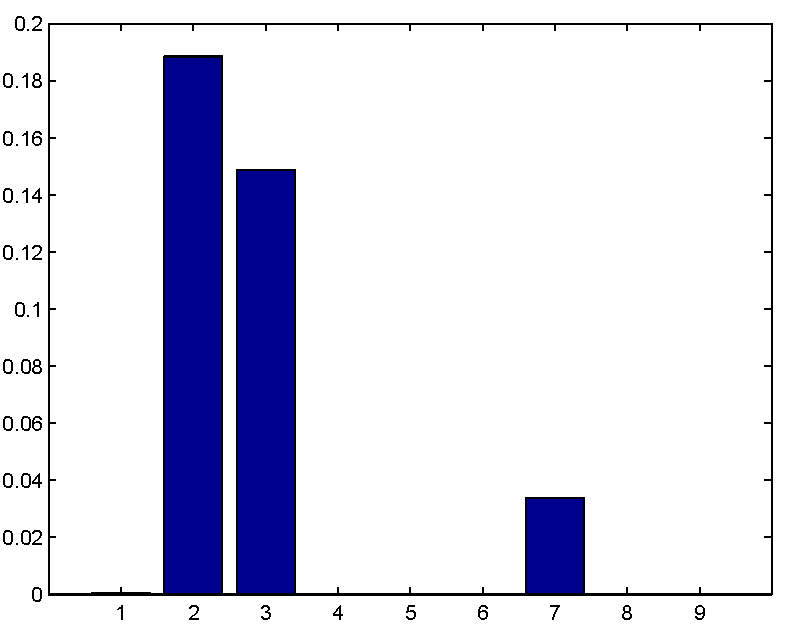
\includegraphics[width=0.4\textwidth]{../diagrams/supplMocapScalesRbf}
	\label{fig:suppMocap1}
}
\subfigure[]{
	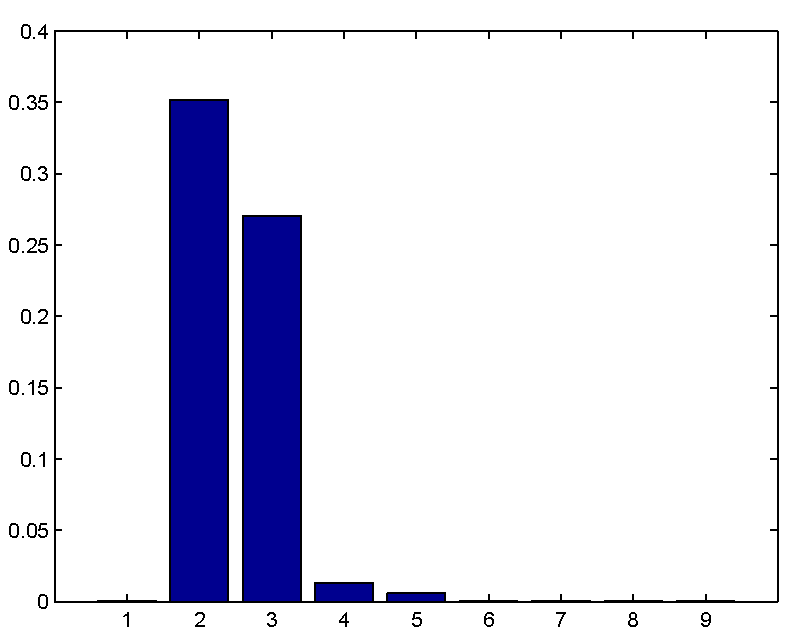
\includegraphics[width=0.4\textwidth]{../diagrams/supplMocapScalesMatern}
	\label{fig:suppMocap2}
}
\end{center}
\caption{\small{
The values of the scales of the ARD kernel after training on the motion capture dataset using the RBF (fig: \subref{fig:suppMocap1}) and the Matern (fig: \subref{fig:suppMocap2}) kernel to model the dynamics for VGPDS. The scales that have zero value ``switch off'' the corresponding dimension of the latent space. The latent space is, therefore, 3-D for \subref{fig:suppMocap1} and 4-D for \subref{fig:suppMocap2}. Note that the scales were initialized with very similar values.
}
}
\label{fig:supplMocap1}
\end{figure}


\begin{figure}[ht]
\begin{center}
\subfigure[]{
	%\includegraphics[width=0.48\textwidth]{diagrams/supplMocapBody23GpdsRbf}
	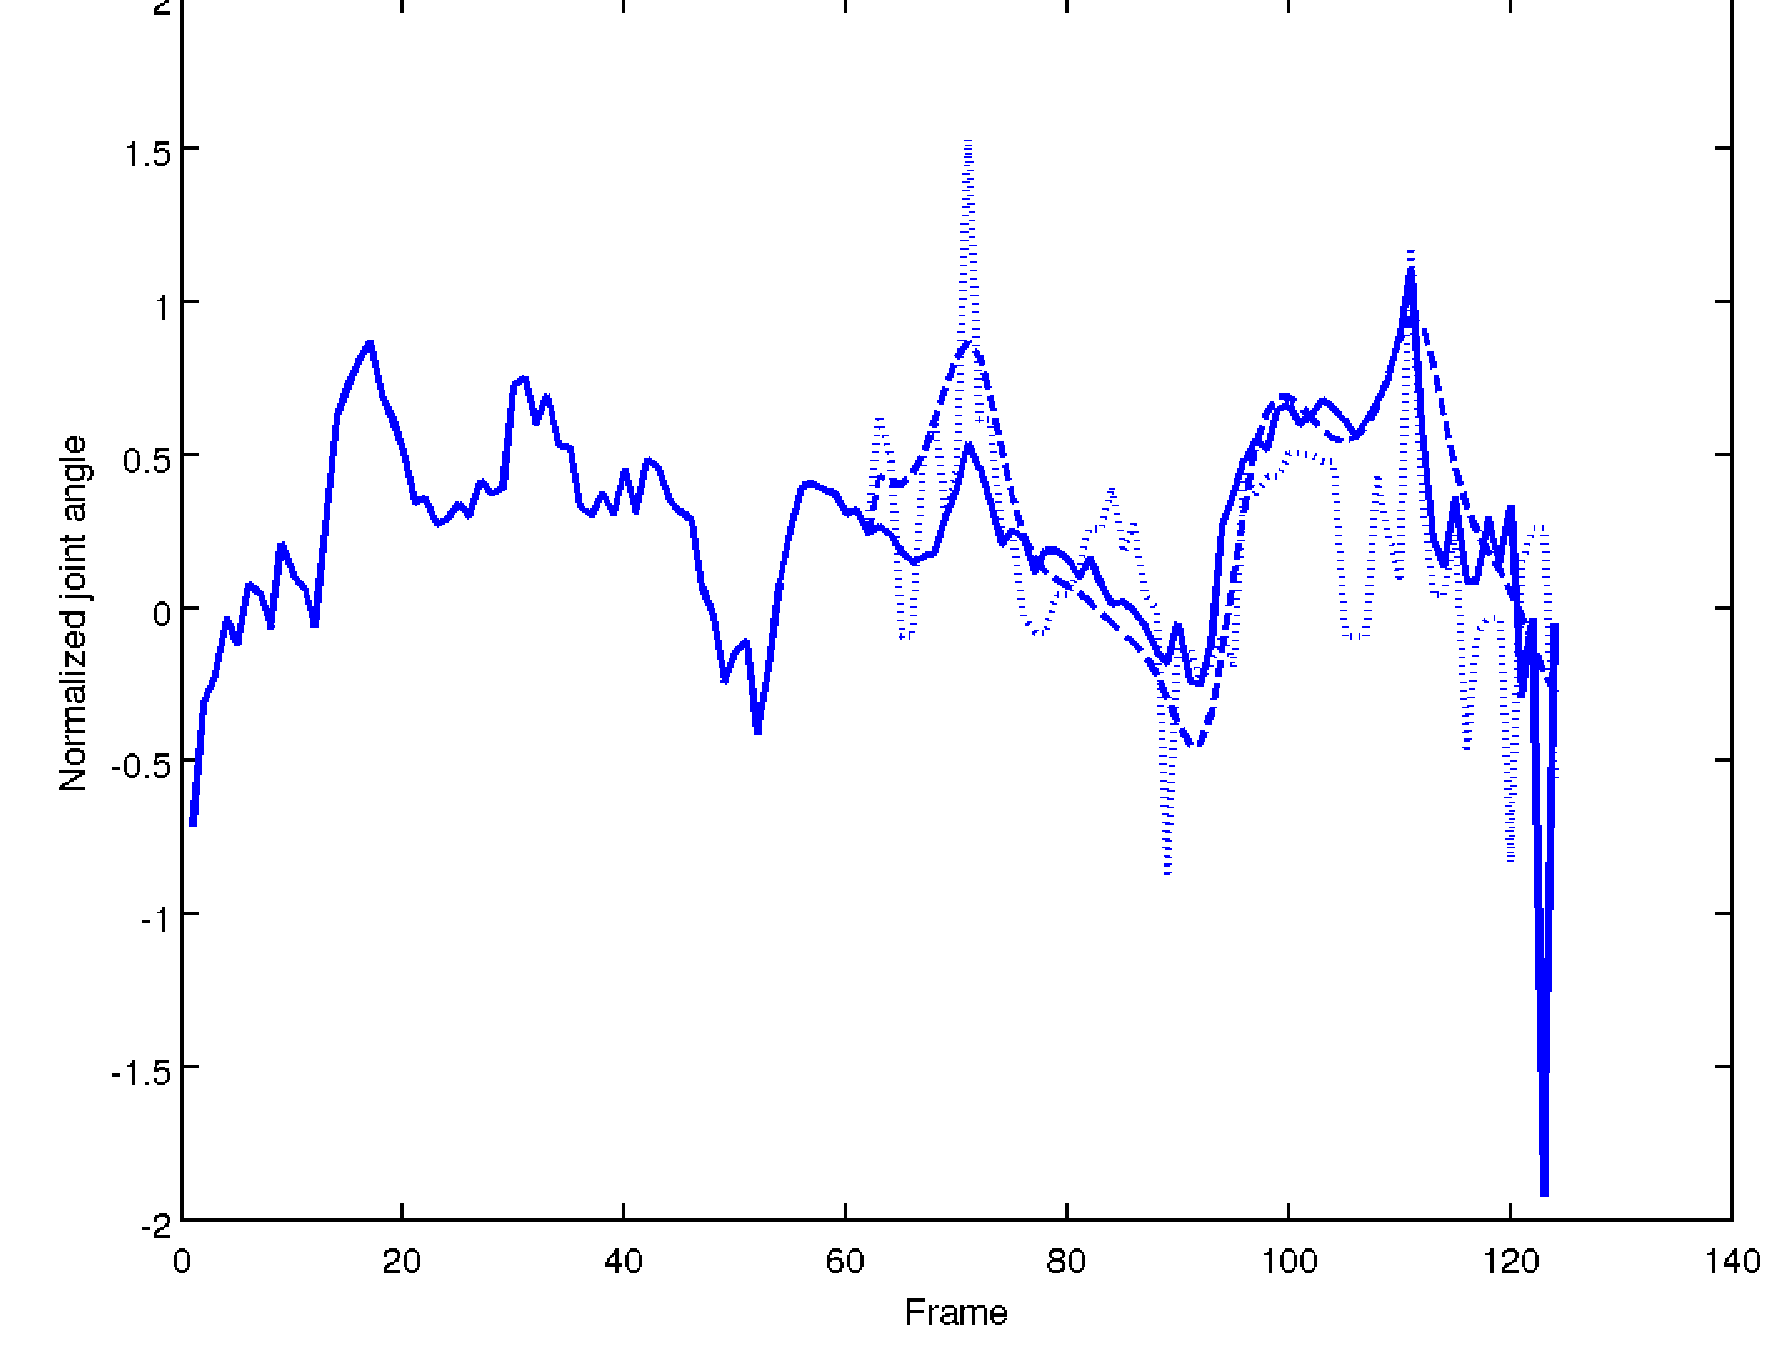
\includegraphics[width=0.48\textwidth]{../diagrams/supplMocapBody28GpdsMatern}
	\label{fig:suppMocap3}
}
\subfigure[]{
	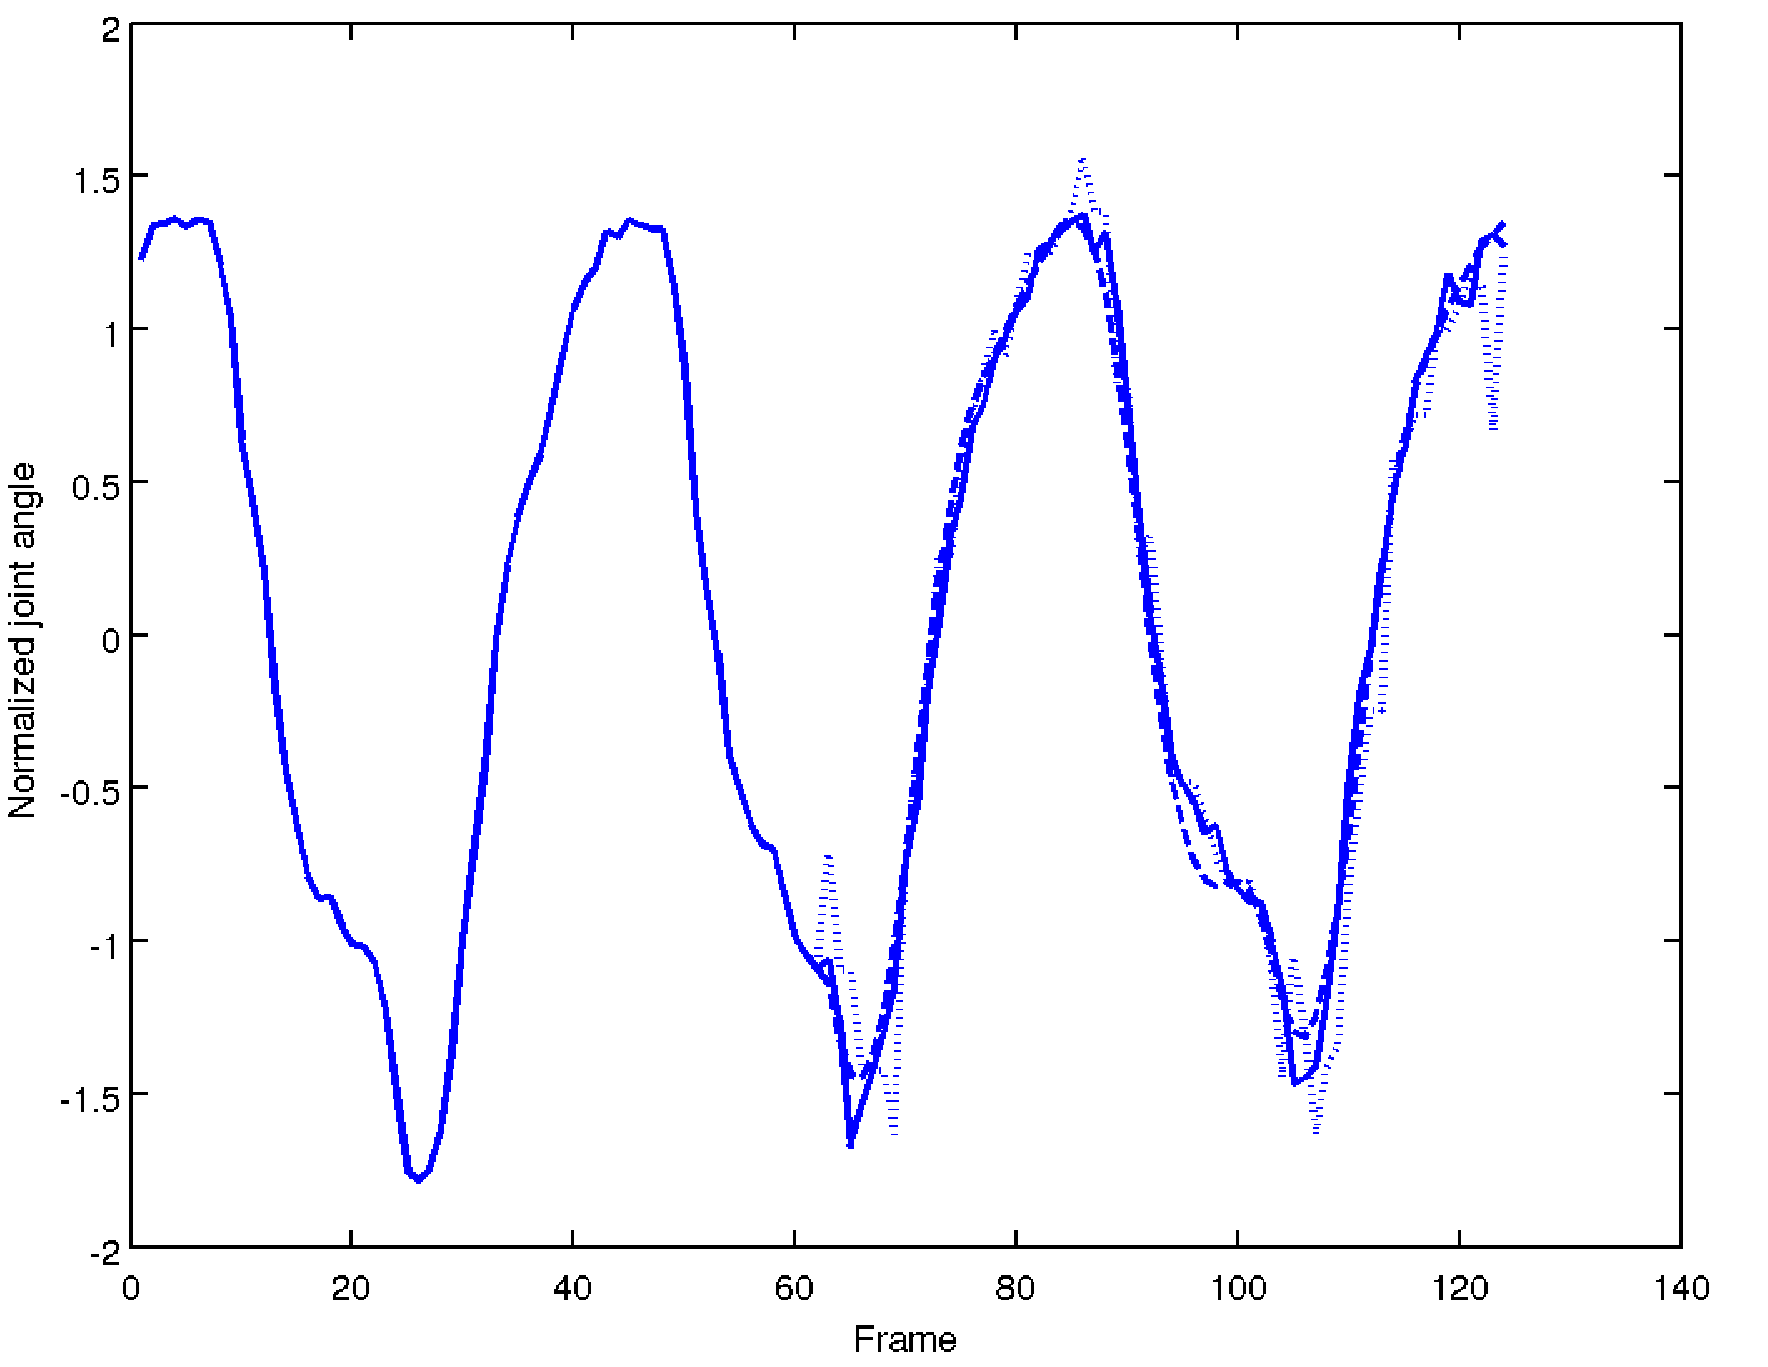
\includegraphics[width=0.48\textwidth]{../diagrams/supplMocapLeg5GpdsMatern}
	\label{fig:suppMocap4}
}
\end{center}
\caption{\small{
The prediction for two of the test angles for the body (fig: \ref{fig:suppMocap3}) and for the legs part (fig: \ref{fig:suppMocap3}). Continuous line is the original test data, dotted line is nearest neighour in scaled space, dashed line is VGPDS (using the RBF kernel for the body reconstruction and the Matern for the legs).
}
}
\label{fig:supplMocap2}
\end{figure}





